% !TeX spellcheck = de_DE

\chapter{Introduction}
The development of modern day software is becoming an increasingly complex activity which warrants extensive research in the field of Software Engineering. According to IEEE Standards, Software Engineering is described as application of a systematic, closely controlled, proven approach to the development, operation and maintenance of software. Along these lines, several methodologies were introduced to reduce the cost and time of software development and to improve the quality of software product. Most of the current research in the field of Software Engineering focuses on some of these objectives and this thesis also tries to address one such purpose.

The first half of this chapter illustrates the motivation behind the thesis work, the problem statement and the proposed solution. The second half illustrates how the thesis is planned and managed along with the organization of the thesis report.
\section{Motivation}
The following section describes the motivation behind the thesis from different perspectives.
\subsection{Software Testing Perspective}
Software Testing is one of the salient steps in the software development lifecycle which ensures whether the developed product meets its purported requirements. Test cases are usually derived from functional requirements, which are usually written in common natural language and this requires a test engineer to manually elicit and develop system test case specifications and then converting it to a test scripting language for automatic execution. Particularly in the context of safety critical systems, the traceability between system test cases and the requirements and the test coverage with respect to requirements are imperative. The efficiency of the manual process depends on the domain expertise of the test engineer and also it does not offer a systematic way to establish test coverage and traceability. Hence it can be stated firmly that the manual process of test case creation is a time consuming, expensive and a non systematic approach. In order to overcome these challenges, this thesis focuses on automatic generation of system test cases directly from requirements specifications written in natural language.
\subsection{Agile Perspective}
Agile software development processes \cite{ambler2009agile} were introduced to keep up with the fast changing marketplace along with the view to support frequent changes in requirements, stakeholder involvement and their priorities and finally quality products with shorter deadlines. Agile development processes have shown greater success rate than traditional software development processes in industry and hence had become an inevitable term in the current software industry. In order to ensure quality products within a shorter development lifecycle, development and testing are done parallel. As requirements changes are frequent in an agile process, the need to change test cases also becomes necessary which when performed manually is time consuming and extensive. Hence an automated process of test case generation plays a huge role in agile development process.
\subsection{Model Based Testing Perspective}
Automatic test case generation has been the topic of study in software engineering for quite a long period. But most of the already proposed approaches need customized artifacts as input for test case generation. For example, \gls{mbt} is one approach in which models of system under test is used for test case generation.  The functional behavior of the system is modeled in any formal specification notations [2] which are then used for the generation of test scenarios and test oracles. The most common artifact used in such cases is the UML models that capture the behavioral or functional aspect of the system. Many approaches require the requirement specifications to be modeled as \glsunset{uml} behavioral models like state charts [3], activity diagrams [4] and sequence diagrams [5].  But these approaches when applied in complex industrial projects require the presence of precise behavioral models representing the system. This again is complex and time consuming process which defeats our core purpose. \gls{mbt} also becomes absurd when an industry never uses formal models in its software development life cycle.  Hence the best approach would be to generate test cases directly from requirement specifications without the need for manual creation of any input artifacts.
\section{Problem Statement}
Software testing is a challenging, time consuming and expensive process in \gls{sdlc}. The process of software testing consists of creation of test cases, test execution and test evaluation. In the mentioned processes, test execution and evaluation is relatively easy and simple whereas creation of test cases utilizes nearly 40 – 70 of the total effort spent on testing [6]. This is because while test execution and evaluation can be easily automated, eliciting test cases from requirements specification and deciding whether the test cases are sufficient to verify the entire system are done manually by testing experts. Such a process of manual elicitation of test cases has the following drawbacks.
\begin{enumerate}
\item The efficiency of the process is hugely dependent on the experience of the testing experts and his knowledge on the particular domain.
\item The process of deriving test cases is not systematic and it solely depends on the experience of the expert.
\item The traceability between requirements and test cases are not systematically established which are necessary for establishing a standard process.
\item There is no standardized process to establish the test coverage and this also leads to the increase in the number of redundant test cases.
\item The requirements written in \gls{nl} are often ambiguous and are interpreted differently by different domain experts. The same holds true for test cases written in \gls{nl} and its interpretation by tester.
\item Finally, the process is manual, error-prone and time consuming.
\end{enumerate}
In order to overcome these drawbacks of the current practices, this thesis focuses on providing an ideal situation where textual, easy to read and traceable test cases are automatically generated from requirements defined in NL. This process should also provide systematic approach for test case generation, ensure necessary test coverage, and provide means to automatically convert these textual test cases into executable test cases along with test input data and thereby improving the quality of the product. In short the thesis tries to address the following questions.
\begin{enumerate}
\item Can we create a tool that can automatically generate test cases from requirements defined in natural language without any intermediate input from domain expert?
\item Can the tool be used to create some intermediate output that can be used in other software engineering process?
\item Can the tool automatically create executable test cases with minimal input from domain experts?
\end{enumerate}
\section{Proposed Solution}
The proposed solution is to create a tool that takes the requirements specification written in natural language as an input and convert it into any intermediate formal notation such as Petri Net. The requirements are usually written as \gls{rucs} which are Use Case Specifications with a defined template and a set of restriction rules. The usage of such rules is to reduce the imprecision and incompleteness in \gls{ucs}. The intermediate \gls{pnm} can be analyzed using any search algorithms for test scenario generation. The test case scenarios are then converted into executable test cases along with test input. The conversion into formal models such as \gls{pnm} has other advantages as it can also be used for other purposes such as checking the completeness, consistency, correctness and unambiguity of the given requirement descriptions [7]. The skeleton of the proposed work is show in Figure \ref{fig:proposed_solution}.
\begin{figure}[htb!]
\centering
\fbox{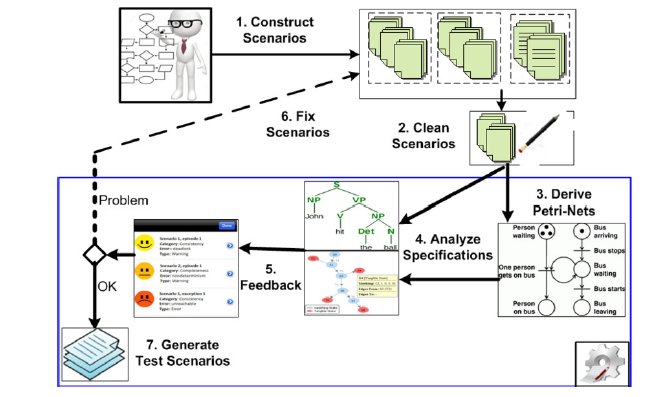
\includegraphics[width=0.8\textwidth]{content/images/proposed_solution.png}}
\caption{An overview of the proposed solution}
\label{fig:proposed_solution}
\end{figure}

\section{Thesis Management}
A project plan was created in order to guarantee an organized approach to this thesis work. Various milestones were created to monitor the progress of the project with time.
\subsection{Project Plan}
A Waterfall model with overlapping phases was created for project planning. The Gantt chart in Figure \ref{fig:gc} shows the various phases and the time duration planned for each phase. 
The significant phases are enlisted below.
\begin{enumerate}
\item Literature Survey
\item Design and Development
\item Testing and further development
\item Documentation
\end{enumerate}
From the Gantt chart it can be seen some phases are overlapped. For example, the overall design of the approach and tool selection for implementation can be made immediately once a feasible approach has been identified in the literature survey. The identification of a suitable system and the enumeration of requirements for basic functionalities of the proposed tool can be done in parallel to the above mentioned phase.
\begin{figure}[htb!]
\centering
\fbox{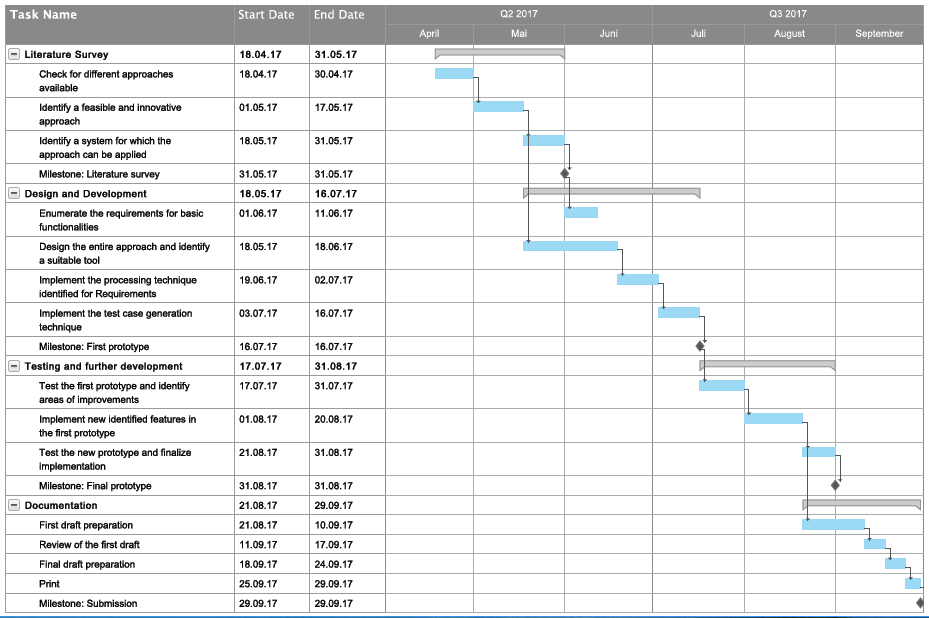
\includegraphics[width=1.05\textwidth]{content/images/figure_2_ganntchart}}
\caption{Gannt Chart for the thesis work}
\label{fig:gc}
\end{figure}
\subsection{Literature Survey}
This thesis mainly revolves around the work done by Edgar et. al., 2015 [8], Wang et. al., 2015 [9] and Toa Yue et. al., 2015 [10]. The literature survey started with the books from the Library of University Stuttgart and moved towards online resources like the IEEE Xplore catalogue, the ACM digital library, the E-Books from various publishers like Springer, the search engines from Internet such as Google \footnote{https://www.google.de} and specific search engines for scientific journals like Google Scholar \footnote{https://scholar.google.de}. Apart from the scientific journals and publications, numerous other resources had been used from internet regarding availability of different tools, their user manuals and their documentation.
\subsection{Thesis Structure}
The thesis has been organized as the following chapters.
\paragraph{Chapter 1} This chapter gives a short introduction to the thesis work, the motivation behind the thesis and a rough idea on the proposed solution.
\paragraph{Chapter 2}